\chapter{Отчет НИР сотрудника ОМИ ДФИЦ РАН Рамазанова М.К. за 2022 г.}


\section*{Аннотация}

Методом Монте-Карло получены магнитные структуры основного состояния двумерной модели Поттса с числом состояний спина $q = 4$ на гексагональной решетке с учетом взаимодействий первых и вторых ближайших соседей во внешнем магнитном поле $h$. Установлено, что в интервалах значений магнитного поля $0 < h < 1.0$ и $2.0 \leq h \leq 3.5$ наблюдается фазовый переход первого рода, а при значении поля $h = 1.5$ --- фазовый переход второго рода. Показано, что в интервале $4.0 \leq h \leq 7.0$ магнитное поле снимает вырождение основного состояния, и фазовый переход размывается.


\section*{Введение}

В течении последних десятилетий наблюдается повышенный интерес к изучению эффектов фрустрации в спиновых решеточных моделях. Конкуренция обменных взаимодействий может привести в магнитных спиновых системах к возникновению фрустрации, которые не позволяют системе одновременно минимизировать все ее локальные взаимодействия, что приводит к бесконечно вырожденному основному состоянию \cite{rmk-bib-1}. Спиновые системы с фрустрациями обладают богатой природой фазовых переходов (ФП) и имеют особенности магнитного, термодинамического и критического поведения. Особый интерес имеет изучение влияния возмущений различной природы, таких как внешнее магнитное поле, взаимодействие вторых ближайших соседей, немагнитные примеси, тепловые и квантовые флуктуации и др. на физические свойства магнитных спиновых систем с фрустрациями. Включение этих возмущающих факторов может привести к совершенно новому физическому поведению таких систем \cite{rmk-bib-2}.

В связи с этим, нами изучается влияние внешнего магнитного поля на характер ФП, магнитные и термодинамические свойства двумерной модели Поттса с фрустрациями. Для фрустрированной модели Поттса существует совсем немного надежно установленных фактов. Большинство имеющихся результатов получены для двумерной модели Поттса с числом состояний спина $q = 2$ и $q = 3$ \cite{rmk-bib-3}. Эта модель изучена достаточно хорошо и получены интересные результаты. Модель Поттса демонстрирует температурный ФП первого или второго порядка, в зависимости от числа состояний спина q, пространственной размерности и геометрии решетки. Двумерная модель Поттса с числом состояний спина $q = 4$ довольно уникальна и до сих пор малоизучена. Результаты исследований двумерной ферромагнитной модели Поттса с числом состояний спина $q = 4$ на треугольной, гексагональной решетках и на решетке Кагоме, полученные методом Монте-Карло (МК) показывают, что в данной модели наблюдается ФП первого рода.

Интерес к модели Поттса обусловлен еще и тем, что эта модель служит основой теоретического описания широкого круга физических свойств и явлений в физике конденсированных сред. К их числу относятся некоторые классы адсорбированных газов на графите, сложные анизотропные ферромагнетики кубической структуры, спиновые стекла, многокомпонентные сплавы и жидкие смеси. На основе модели Поттса с различным числом состояний спина могут быть описаны структурные ФП во многих материалах.

Работ, посвященных изучению влияния внешнего магнитного поля, как возмущающего фактора, на ФП, магнитные и термодинамические свойства модели Поттса с числом состояний спина $q = 4$ практически нет, и этот вопрос все еще остается открытым и малоизученным. В связи с этим, в данной работе нами основе метода МК изучено влияние внешнего магнитного поля на ФП, магнитные и термодинамические свойства двумерной модели Поттса с числом состояний спина $q = 4$ на гексагональной решетке с учетом обменных взаимодействий первых и вторых ближайших соседей. Исследования проводятся на основе современных методов и идей, что позволит получить ответ на ряд вопросов, связанных с характером и природой ФП фрустрированных спиновых систем.


\section{Результат исследования}

Получена фазовая диаграмма зависимости параметра порядка $m$ от величины магнитного поля $h$ в низкотемпературной области (рис. \ref{rmk-fig-1}). На рисунке мы наблюдаем ступенчатую зависимость параметра порядка. Наблюдаются четыре ступеньки: I, II, III и IV. Ступенька I соответствует магнитному упорядочению, при котором только одно состояние спина совпадает с направлением внешнего поля. При увеличении внешнего магнитного поля ($h = 1.5$) еще одно состояние спина выстраивается вдоль внешнего поля. В системе возникает частичный порядок. Это приводит к возникновению ступеньки II на графике. При дальнейшем увеличении поля ($h = 3.0)$, вдоль внешнего поля выстраивается еще одно состояние спина (третье). Этим обусловлено возникновение ступеньки III на графике. При значении поля $h = 4.5$, вдоль внешнего поля выстраивается следующее состояние спина (четвертое). С этим связано возникновение ступеньки IV на графике \cite{rmk-bib-4}.
\begin{figure}[h]
    \begin{center}
        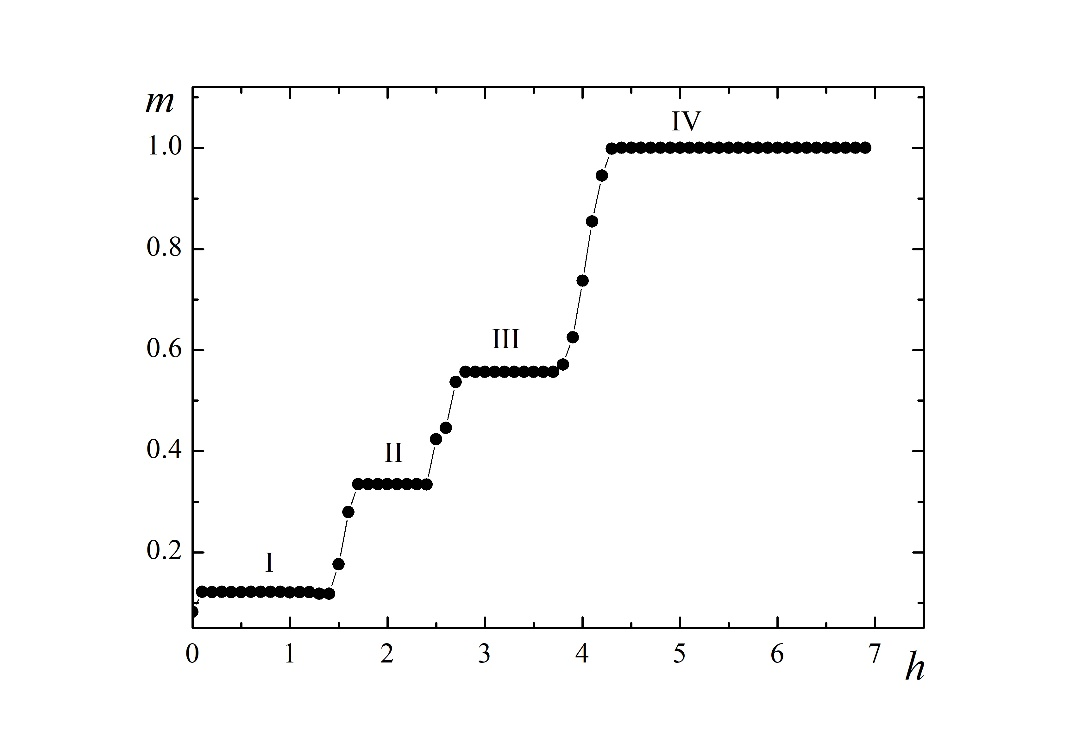
\includegraphics[width=0.75\textwidth]{rmk/image1.jpeg}
    \end{center}
    \caption{Фазовая диаграмма зависимости параметра порядка $m$ от магнитного поля.}
    \label{rmk-fig-1}
\end{figure}

Анализируя рис. \ref{rmk-fig-1} можно предположить, что поля $h = 1.5$; $2.5$ и $4.0$ являются для данной модели фрустрирующими полями. Это также подтверждается поведением температурной зависимости теплоемкости. Теплоемкость в этих полях пологая и значительно ниже, чем в остальных (нефрустрирующих) полях \cite{rmk-bib-4, rmk-bib-5}.


\section*{Заключение}

Исследование влияния магнитного поля на фазовые переходы, магнитные структуры основного состояния и термодинамические свойства двумерной модели Поттса с числом состояний спина $q = 4$ на гексагональной решетке с взаимодействиями вторых ближайших соседей выполнено с использованием репличного обменного алгоритма метода Монте-Карло. На основе гистограммного метода проведен анализ характера фазовых переходов. Получены магнитные структуры основного состояния в широком интервале значений поля. Построена фазовая диаграмма зависимости параметра порядка от величины магнитного поля. Показано, что в интервале значений магнитного поля $0.0 \leq h \leq 3.5$, кроме значения $h = 1.5$ наблюдается фазовый переход первого рода. Для поля $h = 1.5$ наблюдается фазовый переход второго рода. Обнаружено, что при сильных полях $h \geq 4.0$ магнитное поле снимается вырождение основного состояния и фазовый переход в системе размывается.
